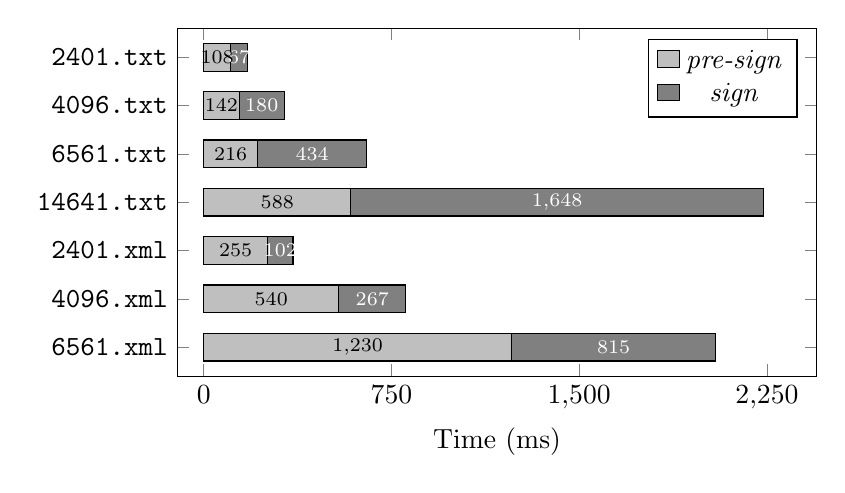
\begin{tikzpicture}
    \begin{axis}[
        width=.8\textwidth,
        height=6cm,
        xbar stacked,
        nodes near coords,
        legend pos=north east,
        xlabel={Time (ms)},
        xtick={0, 750, 1500, 2250},
        symbolic y coords = {
            6561.xml,
            4096.xml,
            2401.xml,
            14641.txt,
            6561.txt,
            4096.txt,
            2401.txt,
        },
        ytick=data,
        y tick label style={font=\ttfamily},
        nodes near coords style={black, font=\scriptsize}
    ]
        \addplot+[
            xbar,
            black,
            fill=lightgray,
        ] plot coordinates {
            (108,2401.txt)
            (142,4096.txt)
            (216,6561.txt)
            (588,14641.txt)
            (255,2401.xml)
            (540,4096.xml)
            (1230,6561.xml)
        };
        \addlegendentry{\textit{pre-sign}}
        
        \addplot+[
            xbar,
            black,
            fill=gray,
            nodes near coords style={white, font=\scriptsize},
        ] plot coordinates {
            (67,2401.txt)
            (180,4096.txt)
            (434,6561.txt)
            (1648,14641.txt)
            (102,2401.xml)
            (267,4096.xml)
            (815,6561.xml)
        };
        \addlegendentry{\textit{sign}}
    \end{axis}
\end{tikzpicture}